\newcommand{\dirname}{\lstinline'sample-handout'}
\newcommand{\tgzname}{\dirname \lstinline'.tgz'}

\section*{Completing a Programming Assignment}

In this section, we'll walk through the steps of downloading,
completing, and submitting a programming assignment. You'll do this
for each assignment, so come back here if you get confused.

You will be primarily using the command \lstinline'autolab122' to
interact with \autolab{}.  You can also use the \autolab{} web site
(\href{\autolabURL}{\autolabURL}) if you prefer.


\begin{part}\TAGS{unix}
To begin with, you need to do a one-time setup for \lstinline'autolab122'.
Simply run
\begin{lstlisting}[language={[coin]C}]
% autolab122 setup
\end{lstlisting}\vspace{-1.5ex}
and follow the instructions.  You will not need to do this again.
Here's a sample interaction.
\begin{center}
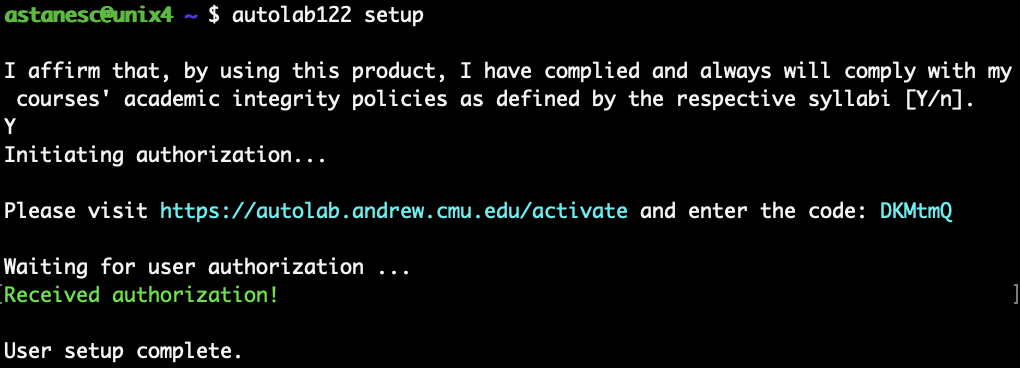
\includegraphics[width=0.75\linewidth]{\img/autolab122-setup.png}
\end{center}
\end{part}


\begin{part}\TAGS{unix}
  Make sure you are in the \lstinline[language={[coin]C}]'private/15122'
  directory by entering the command
  \underline{\lstinline[language={[coin]C}]'pwd'} to get the
    \textbf{\color{red}p}resent
  \textbf{\color{red}w}orking \textbf{\color{red}d}irectory. You should see something like this with your andrew id
  instead of \lstinline[language={[coin]C}]'<your_id>':

\begin{lstlisting}[language={[coin]C}]
% pwd
/afs/andrew.cmu.edu/<usr_number>/<your_id>/private/15122
\end{lstlisting}\vspace{-1.5ex}
If you ever get lost, you can go there by entering
\begin{lstlisting}[language={[coin]C}]
% cd
% cd private/15122
\end{lstlisting}\vspace{-1.5ex}
\end{part}


\begin{part}\TAGS{unix}
  You can list the currently released assignments by running
\begin{lstlisting}[language={[coin]C}]
% autolab122 hw
  sample (Sample Assignment (UNGRADED))
\end{lstlisting}\vspace{-1.5ex}
You will see the assignment called \lstinline'sample' --- the
description in parentheses is for your information only --- and
possibly other material we are distributing through \autolab{}.  You
will be using this name (\lstinline'sample') when interacting with
Autolab about this assignment.
\end{part}


\begin{part}\TAGS{unix}
  Download the starter code for assignment \lstinline'sample' with
  the following command:
\begin{lstlisting}[language={[coin]C}]
% autolab122 download sample
Querying assessment 'sample' of course '15122-[*\shortsem*]' ...
Creating directory /home/iliano/TMP/sample
Handout downloaded into assessment directory
Writeup downloaded into assessment directory

Due: Mon Jun 29 18:00:00 2020
sample successfully downloaded.
\end{lstlisting}\vspace{-1.5ex}
This creates a directory called \lstinline'sample' with the following
contents:
\begin{lstlisting}[language={[coin]C}]
% ls sample
factorial.c0  favorite_number.c0  README.txt
\end{lstlisting}\vspace{-1.5ex}
The file \lstinline'README.txt' tells you how to compile the
assignment and how to submit it.  The other files are what you'll be
working on.
\end{part}




\subsection*{Editing your program}

You can use any editor you wish to write and edit your programs, but
we highly recommend you try out
\lstinline[language={[coin]C}]'VSCode',
\lstinline[language={[coin]C}]'vim', or
\lstinline[language={[coin]C}]'emacs'. These editors are very powerful
and can do much more than just help you edit your code (as you will see).

All three are pre-installed on the GHC cluster computers.

You can also use them from your own computer.  To use
\lstinline[language={[coin]C}]'vim' or
\lstinline[language={[coin]C}]'emacs', you will need to ssh in to one
of the Linux andrew machines; once there, you simply run them
from the terminal prompt as described below.  To use the more modern
\lstinline[language={[coin]C}]'VSCode', you will first need to install
it on your computer by following the few easy steps in the ``VSCode
Guide'' on \gts{} under ``Guides to Success''.


% When ssh'd in to one of the Linux andrew machines,
% \lstinline[language={[coin]C}]'vim' and
% \lstinline[language={[coin]C}]'emacs' can be run directly from the
% terminal without additional setup.  If you prefer working with a more
% modern code editor directly on your own computer, you can set up
% \lstinline[language={[coin]C}]'VSCode' by following a few easy steps
% on the ``VSCode Guide'' on \gts{} under ``Guides to Success''.

For this section of the lab handout, we provide instructions on
working with \lstinline[language={[coin]C}]'VSCode',
\lstinline[language={[coin]C}]'vim' and
\lstinline[language={[coin]C}]'emacs'. We highly recommend that you
\textbf{try all three of them}.  Later, use the one you like
best\footnote{See the
  \href{http://www.cs.cmu.edu/~15122/about.shtml}{course website}
  to learn more about using these editors. They are capable
  of much more than what we describe here.}.

\begin{part}\TAGS{unix}
  Using \underline{\lstinline'cd'}, go into the \lstinline'sample' directory.
  From there open the file \lstinline[language={[coin]C}]'factorial.c0'
  that you downloaded from the previous part of the lab:

  \begin{minipage}[t]{0.4\linewidth}
    \textbf{VIM:}\\ \lstinline[language={[coin]C}]'% vim factorial.c0'

    \medskip
    \textbf{EMACS:}\\ \lstinline[language={[coin]C}]'% emacs factorial.c0'
  \end{minipage}
  % \begin{minipage}[t]{0.3\linewidth}
  %   \textbf{EMACS:}\\ \lstinline[language={[coin]C}]'% emacs factorial.c0'
  % \end{minipage}
  \begin{minipage}[t]{0.5\linewidth}
    \textbf{VSCode:}\\ Start the ``Visual Studio Code'' application and
    open the file \lstinline'factorial.c0' from its ``File'' menu.
  \end{minipage}
\end{part}

You should see the editor start in the Terminal or a \lstinline'VSCode'
window, and you should see a program that looks like it computes
factorial\footnote{For \textbf{Emacs} or \textbf{vim}, trying
  to open a file that doesn't exist (i.e., by making a typo) will create
  a new empty file with that name. If you see a blank file, exit the editor
  and try again.}.
The program is written in C0, the language we'll be using
to start the semester.

\begin{part}\TAGS{unix}
  Edit the program \lstinline[language={[coin]C}]'factorial.c0' and add your
  name and section letter at the appropriate locations. Use the instructions
  below for the editor you're using.

  \textbf{VIM:} This editor has two modes -- \emph{insert mode} for inserting
  text or code, and \emph{command mode} for entering commands. It starts in
  command mode, so you can't edit immediately. Use the arrow keys to
  move around the file. While in command mode, pressing ``\lstinline'i'''
  changes the editor to insert mode, allowing you to type text. Go into
  insert mode and add your name and section letter.
  Press the Escape (ESC) key while in insert mode to return
  to command mode.

  \textbf{EMACS:} You can just start typing and editing without
  hitting special keys. You can use the arrow keys to navigate around
  the file to insert code. There are many shortcuts and built-in
  features to Emacs but you won't need them right now. In the file,
  insert your name and your section letter in the appropriate
  comments in your program.

  \textbf{VSCode:} You can just start typing and use your mouse or
  arrow keys to move around the file. Insert your name and
  section letter in the appropriate comments in your program.
\end{part}

\begin{part}\TAGS{unix}
  Save your changes and exit the editor.

  \textbf{VIM:} Make sure you're in command mode by pressing ESC\@.
  Then, you can save your work and exit vim by entering the
  sequence ``\lstinline':wq''' followed by pressing Enter.
  (If you have unsaved changes you would like to discard,
  you'll have to enter the sequence ``\lstinline':q!''' followed by Enter.
  You can also save without exiting by entering the sequence
  ``\lstinline':w''' followed by Enter.)

  \textbf{EMACS:} Once you're ready to save, press Ctrl-x (the Control
  key and the ``\lstinline'x''' key at the same time) followed by
  Ctrl-s. You can exit by pressing Ctrl-x followed by Ctrl-c.  If you
  have not saved before exiting, Emacs will ask you whether you want
  to save your file (since you changed it) --- press ``\lstinline'y'''
  for yes. (Press ``\lstinline'n''' instead if you don't want to save
  your changes).

  \textbf{VSCode:} To save your work, simply select ``Save'' from the
  ``File'' menu. If you use VSCode regularly, you will want to learn
  some of the shortcuts for common commands, for example Ctrl-s or Cmd-s
  to save a file.

\end{part}

\begin{part}\TAGS{unix}
Try out your new editing skills on the file \lstinline'favorite_number.c0'.
You should see where the file tells you to add a line that returns your
favorite number, like this:
\begin{lstlisting}[language={[coin]C}, belowskip=0pt]
int my_favorite_number() {
    /* add a line below that returns your favorite number */
    return 17; // this is *my* favorite number. Choose your own.
}
\end{lstlisting}
\end{part}

\subsection*{Running a C0 Program}

You can execute a C0 program by either compiling it into executable
code or loading it into an interpreter. You invoke the C0 compiler
(\lstinline[language={[coin]C}]'cc0') and interpreter
(\lstinline[language={[coin]C}]'coin') from the Linux command line.

The \emph{compiler} translates your program into a lower level
(machine) version of the code that can be executed by the computer.
It first checks for syntax errors and will abort with an error message
if it finds any.

\begin{part}\TAGS{compilation}
  Be sure you're in the \lstinline'sample' directory, then 
  \textbf{\color{red}c}ompile your \textbf{\color{red}c0} code using the
  \lstinline[language={[coin]C}]'cc0' compiler:
\begin{lstlisting}[language={[coin]C}, belowskip=0ex]
   % cc0 -d factorial.c0
\end{lstlisting}
This runs the compiler with debug mode on
(\lstinline[language={[coin]C}]'-d').  During execution, the debug
mode checks all the code annotations starting with \lstinline'//@'.
You will learn about them in class.
\end{part}
\vspace{-1ex}

If there are no syntax errors, the \lstinline[language={[coin]C}]'cc0'
compiler returns to the command prompt without saying anything else.
Running \underline{\lstinline[language={[coin]C}]'ls'} will show you a
new file named \lstinline[language={[coin]C}]'a.out', which is the
executable version of your program. If you have syntax errors during
compilation, go back into the file with an editor and correct them.

%\enlargethispage{5ex}
\begin{part}\TAGS{compilation, unix}
  Run the program:
\begin{lstlisting}[language={[coin]C}, belowskip=0ex]
  % ./a.out
\end{lstlisting}
The first dot says to look in the current directory and run the
\lstinline[language={[coin]C}]'a.out' executable file. This will cause
the \lstinline'main()' function in your program to launch, which
prints the values of $0!$ through $9!$ in the terminal window, one per
line.
\end{part}
\vspace{-1ex}

%This shows how to \emph{compile} and \emph{run} your programs.
Alternatively, you can use the \textbf{\color{red}C0}
\textbf{\color{red}in}terpreter \lstinline[language={[coin]C}]'coin' to execute
your program. An \emph{interpreter} checks a program for syntax errors
%, translates it into machine code, and runs the resulting code
and runs it step by step.  This is a good way to interact with your
program in real time to test it.

\begin{part}\TAGS{interpreter}
  Run your program in the \lstinline[language={[coin]C}]'coin'
  interpreter, starting it with %
  \lstinline[language={[coin]C}]'coin -d factorial.c0' %
  and entering in the C0 statements as shown below.
\begin{lstlisting}[language={[coin]C}, belowskip=-2ex]
  % coin -d factorial.c0
  C0 interpreter (coin)
  Type `#help' for help or `#quit' to exit.
  --> factorial(2);
  --> factorial(3);
\end{lstlisting}
%  --> factorial(4);
%  --> factorial(10);
%  --> factorial(17);
\end{part}
Exit the interpreter by entering \lstinline[language={[coin]C}]'#quit' and
pressing Enter, or using the keyboard shortcut Ctrl-d.

\begin{comment}
Some of the outputs \lstinline[language={[coin]C}]'coin' gives should
strike you as odd. We'll learn about what's going on in class.

\begin{part}\TAGS{intepreter}
  Factorial $n!$ is only defined on non-negative numbers. Try to
  compute a non-existent factorial:
\begin{lstlisting}[language={[coin]C}, belowskip=-1.5ex]
  --> factorial(-1);
\end{lstlisting}
\end{part}

You should see an annotation failure.  This is because our factorial
function starts with the requirement: \lstinline'//@requires n >= 0;'.
Since we called this function with a value for $n$ that does not
satisfy this requirement, we get an annotation failure since it
doesn't make sense to run this function with $n = -1$.

\begin{part}\TAGS{intepreter}
  Exit the interpreter by entering
  \lstinline[language={[coin]C}]'#quit'.  Start it again, this time without the
  \lstinline[language={[coin]C}]'-d' flag by typing
  \lstinline[language={[coin]C}]'coin factorial.c0' at the prompt.  Now, run
  \lstinline[language={[coin]C}]'factorial(-1);' again.  What do you observe?
\end{part}
\end{comment}



\subsection*{Submitting Programming Assignments}

\begin{part}
You will submit the assignment by typing the following
at the Unix prompt:
\begin{lstlisting}[language={[coin]C}]
% autolab122 handin sample factorial.c0 favorite_number.c0
\end{lstlisting}\vspace{-1.5ex}
The command to type is always written at the bottom of the file
\lstinline'README.txt' that comes with each assignment.

This command will ask you to acknowledge the academic integrity policy
of the class and then submit the files to \autolab{}.  Once \autolab{}
is done grading this submission, it will display your scores.  Here's
the full output:
\begin{lstlisting}[language={[coin]C}, deletekeywords={for},
  deletedelim={[l]{Type\ }}, deletestring={[b]{'}}]
% autolab122 handin sample factorial.c0 favorite_number.c0
Type "yes" to affirm that you have complied with this course's
academic integrity policy as defined in the syllabus: yes
Submitting to 15122-[*\shortsem*]:sample ... (force)
Successfully submitted to Autolab (version 1)

Waiting for scores to be ready ...
Scores for 15122-[*\shortsem*]:sample
 version | handin (1.0) | editing (1.0) |
+---------+--------------+---------------+
|       1 |          1.0 |           0.0 |
\end{lstlisting}

At this point, you can see the overall \autolab{} feedback with
\begin{lstlisting}[language={[coin]C}]
% autolab122 feedback
\end{lstlisting}
\chkptB
\end{part}
